\subsubsection{\textit{Git}}

Basicamente, o \textit{Git} é um sistema distribuído e de código aberto que controla versões de arquivos desenvolvidos, no qual possui diversos comandos que auxilia os desenvolvedores a realizar projetos de grade e pequeno porte com velocidade e eficiência.  Com esses comandos, o \textit{Git} disponibiliza um amplo conjunto de ferramentas para realizar a manipulação dos arquivos no seu repositório local ou \textit{Web}, garantindo a integridade dos dados \cite{GIT2010}.

A \autoref{fig_git} demostra um exemplo da utilização de comandos \textit{git} para controlar um repositório local ou \textit{web}.

\begin{figure}[h]
	\caption{\label{fig_git}Exemplo de comandos \textit{Git}.}
	\begin{center}
		\resizebox{1\linewidth}{!}{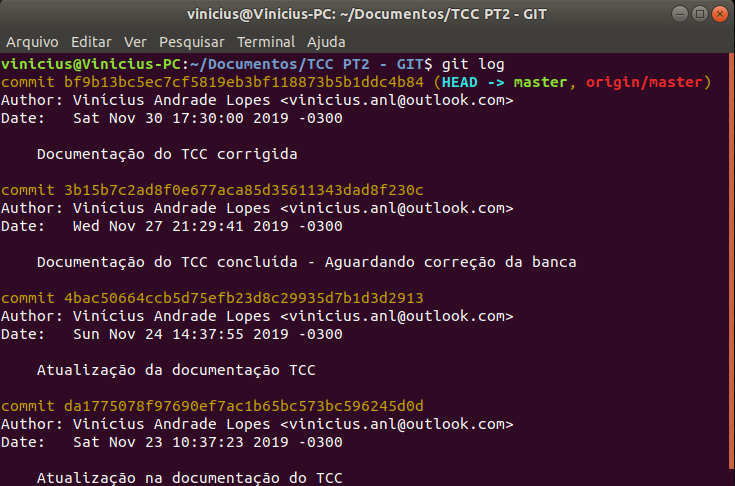
\includegraphics{4-Conteudo-Bibliografico/4-Ferramentas-de-Desenvolvimento-do-Projeto/git.png}}
	\end{center}
	\centering \legend{Fonte: Elaborada pelos autores.}
\end{figure}

Segundo \citeonline{CHACON2014}, o maior diferencial do sistema de controle de versões \textit{Git} é o seu modelo de ramificação (\textit{branch}), que possibilita ao usuário a criação de uma cópia do sistema principal. Com essa cópia, o desenvolvedor pode realizar implementações de melhorias/correções em trechos de códigos sem modificar a aplicação principal. Depois da implementação e dos testes, o desenvolvedor pode substituir a \textit{branch} principal (\textit{master}) pela \textit{branch} com implementações. Os únicos arquivos que serão substituídos serão os arquivos editados.